% !TEX encoding = UTF-8
% !TEX TS-program = pdflatex
% !TEX root = ../tesi.tex

%**************************************************************
\chapter{Descrizione dello stage}
\label{cap:descrizione-stage}
%**************************************************************

\section{Vantaggi per l'azienda}
WebPD trae diversi vantaggi dall'attività di stage curricolare che è stata disposta ad ospitare.\\
\\
Primo su tutti, l'inserimento in azienda, seppur solo per un paio di mesi, di un nuovo membro del personale, mai entrato in contatto con l'azienda. Ciò, in primis, ha permesso di distribuire il carico di lavoro tra più persone, permettendo di accelerare lo sviluppo sui progetti in cantiere. Inoltre, l'introduzione nel team di una persona completamente esterna all'azienda, ha portato un ulteriore punto di vista all'interno del team di sviluppo. Tale punto di vista si è dimostrato utile nel tentativo di risoluzione di alcuni problemi software "cronici" (come la lentezza di esecuzione delle query, problema che verrà descritto nel dettaglio nel prossimo capitolo), permettendo un ragionamento fuori dagli schemi mentali dell'ideatore di tale software.\\
\\
In secondo luogo, ha permesso all'azienda di esplorare nuovi canoni stilistici per alcuni suoi prodotti a costo zero, come nel caso del restyling della homepage del sito CrociereRegalo (descritta anch'essa nel prossimo capitolo), senza quindi il rischio di sacrificare inutilmente il lavoro (e la retribuzione) di un membro del personale.

\section{Presentazione del progetto}
L'obiettivo di questo stage è stato permettere a WebPD di completare la riscrittura (da capo) del sito CrociereRegalo.it. Tale sito, infatti, prima dell'ingresso di Primarete tra le quote di WebPD, era stato realizzato e mantenuto da WebCola, una web agency con la quale Primarete aveva stretto una partnership commerciale, che si è appunto interrotta nel 2015.\\
Secondo gli accordi presi, il sorgente del sito era di proprietà di WebCola, pertanto non è stato possibile per WebPD procedere ad una semplice modifica/aggiornamento di qualcosa già esistente. Il vecchio sito, inoltre, non era responsive e, dai dati di Google Analytics é emerso che la maggior parte delle visite avveniva da dispositivi mobili. \\
La problematica maggiore, comunque, erano (e lo sono tuttora) gli accordi presi con le varie compagnie di crociera (MSC, Costa, Royal Caribbean, Celebrity e Azamara): tali accordi, infatti, erano stati presi da WebCola in nome e per conto suo, quindi WebPD si è vista obbligata a ristabilirli.
\begin{figure}[!h] 
	\centering 
	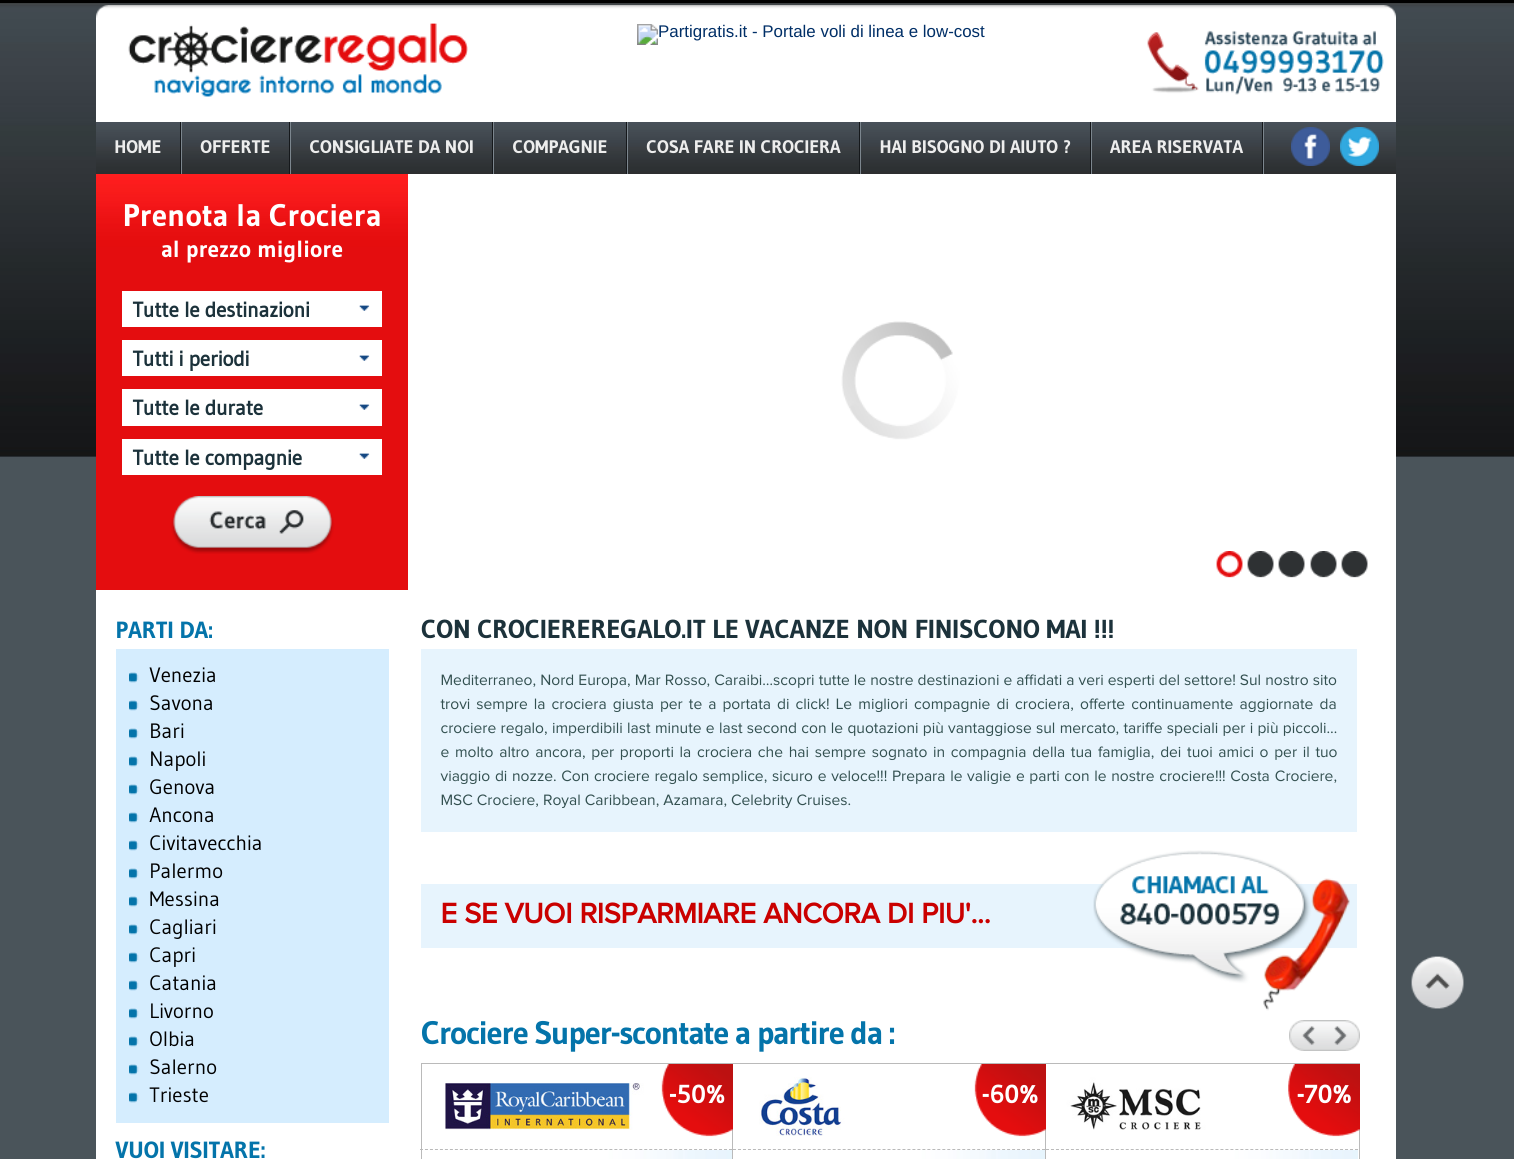
\includegraphics[width=.9\columnwidth]{stage/webcola_crociereregalo} 
	\caption{Screenshot della versione di CrociereRegalo sviluppata da WebCola}
\end{figure}\\
